\documentclass[11pt,a4paper]{article}
\usepackage[T1]{fontenc}
\usepackage[utf8]{inputenc}
\usepackage{lmodern}
\usepackage{textcomp}
\usepackage[left=1.8cm,right=1.8cm,top=3.0cm,bottom=2.2cm,headheight=36pt,headsep=12pt]{geometry}
\usepackage{multicol}
\usepackage{xcolor}
\usepackage{fancyhdr}\usepackage{tikz}
\usepackage{graphicx}
\usepackage{array}
\usepackage{amsmath,amssymb}
\usepackage{setspace}
\usepackage{longtable}
\graphicspath{{../}}
\definecolor{ygreen}{RGB}{46,139,87}\definecolor{dgreen}{RGB}{28,90,56}
\renewcommand{\normalsize}{\fontsize{10.9}{13.4}\selectfont}
\renewcommand{\familydefault}{\rmdefault}
\setlength{\parindent}{0pt}
\setlength{\columnsep}{0.8cm}
\setlength{\columnseprule}{0.4pt}
\setlength{\multicolsep}{3pt plus 1pt minus 1pt}
\renewcommand{\textsubscript}[1]{\ensuremath{_{\text{\fontsize{8}{8}\selectfont #1}}}}
\renewcommand{\textsuperscript}[1]{\ensuremath{^{\text{\fontsize{8}{8}\selectfont #1}}}}
\newcommand{\qn}[1]{\textbf{\fontsize{11.5}{13}\selectfont #1}}
\newcommand{\qsep}{\par\vspace{13pt}}
\newcommand{\fwrule}{\par\vspace{5pt}\noindent\rule{\linewidth}{1.4pt}\par\vspace{7pt}}
\newsavebox{\fitb}
\newcommand{\fitbox}[1]{\sbox{\fitb}{#1}\ifdim\wd\fitb>\linewidth\resizebox{\linewidth}{!}{\usebox{\fitb}}\else\usebox{\fitb}\fi}
\newcommand{\diqqat}[1]{\par\smallskip\noindent\textbf{Diqqat!} #1\par\medskip}
\newcommand{\javob}{\par\nopagebreak[4]\smallskip\noindent\textbf{Javob:} \rule[-2pt]{7.5cm}{0.4pt}\par\smallskip\noindent\textbf{Diqqat!} Javobingizni javoblar varaqasiga ko`chirib yozing.\par\medskip}
\pagestyle{fancy}
\fancyhf{}
\renewcommand{\headrulewidth}{1.6pt}\renewcommand{\headrule}{{\color{ygreen}\hrule height 1.6pt width\headwidth}}
\newcommand{\hdrlogo}{
\begin{tikzpicture}[baseline=0pt]\fill[ygreen,rounded corners=3pt] (0,0) rectangle (0.95,0.95);\node[white,font=\fontsize{24}{26}\bfseries\selectfont] at (0.475,0.47){K};\node[anchor=west,font=\fontsize{16}{18}\bfseries\selectfont,text=dgreen] at (1.15,0.66){KIMYO};\node[anchor=west,font=\footnotesize\scshape,text=gray] at (1.15,0.2){Milliy sertifikat\ \ 2026};\end{tikzpicture}}
\newcommand{\hdrpill}[1]{\begin{tikzpicture}[baseline=0pt]\node[fill=ygreen,text=white,rounded corners=8pt,inner xsep=10pt,inner ysep=5pt,font=\fontsize{13}{15}\bfseries\selectfont] at (0,0.475){#1};\end{tikzpicture}}
\fancyhead[L]{\hdrlogo}
\fancyhead[R]{\hdrpill{2-variant}}

\fancyfoot[C]{\thepage}
\fancypagestyle{first}{\fancyhf{}\renewcommand{\headrulewidth}{1.6pt}\renewcommand{\headrule}{{\color{ygreen}\hrule height 1.6pt width\headwidth}}\fancyhead[L]{\hdrlogo}\fancyhead[R]{\hdrpill{2-variant}}\fancyfoot[C]{\thepage}}
\begin{document}
\normalsize
\thispagestyle{first}
\noindent\textit{Davriy jadvaldan foydalanish mumkin.}
\par\smallskip
\begin{multicols}{2}
\noindent\qn{1.} 2-davr elementlari atom radiuslarining o`zgarishi diagrammada ko`rsatilgan.
\begin{center}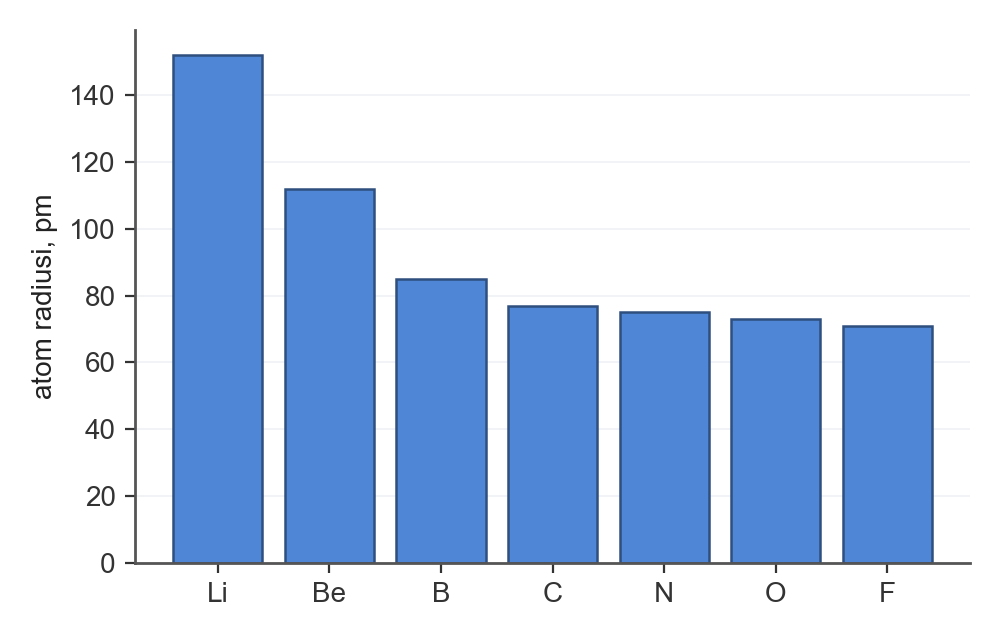
\includegraphics[width=0.86\linewidth]{rasmlar/gen/ra_v02_0.png}\end{center}
Davr bo`yicha chapdan o`ngga atom radiusi qanday o`zgaradi va sababi nima?
\noindent A)~\textsl{Kamayadi, yadro zaryadi ortishi tufayli}\par
\noindent B)~\textsl{Ortadi, qavatlar soni ko`payishi tufayli}\par
\noindent C)~\textsl{Kamayadi, qavatlar soni kamayishi tufayli}\par
\noindent D)~\textsl{O`zgarmaydi}\par
\qsep
\noindent\qn{2.} Quyidagi zarrachalardan qaysilari argon atomi bilan izoelektron? 1) Al\textsuperscript{3+}; 2) O\textsuperscript{2$-$}; 3) K\textsuperscript{+}; 4) Cl\textsuperscript{$-$}

\noindent A)~\textsl{1, 4} \hfill B)~\textsl{2, 3} \hfill C)~\textsl{2, 3, 4} \hfill D)~\textsl{3, 4}\par
\qsep
\noindent\qn{3.} Rasmda radioaktiv yemirilish zanjiri berilgan (massa soni/zaryad; ``?'' -- oraliq yadrolar).
\begin{center}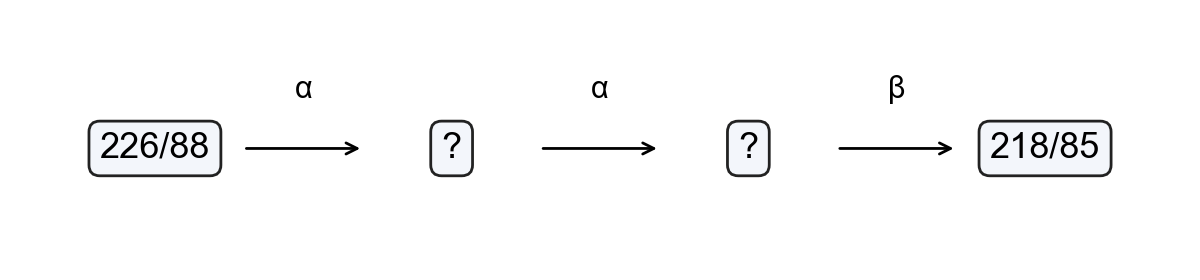
\includegraphics[width=0.86\linewidth]{rasmlar/gen/dc_47498.png}\end{center}
Zanjirda nechta $\alpha$-zarra chiqarilgan?

\noindent A)~\textsl{3} \hfill B)~\textsl{4} \hfill C)~\textsl{2} \hfill D)~\textsl{5}\par
\qsep
\noindent\qn{4.} Zarracha haqida ma'lumot jadvalda berilgan:
\begin{center}
\renewcommand{\arraystretch}{1.15}
\fitbox{\begin{tabular}{|c|c|}\hline
\textbf{Zarracha tarkibi} & \textbf{Soni} \\ \hline
proton & 26 \\ \hline
neytron & 27 \\ \hline
elektron & 25 \\ \hline
\end{tabular}}
\end{center}
Shu zarrachaning massa \textbf{sonini aniqlang.}

\noindent A)~\textsl{53} \hfill B)~\textsl{54} \hfill C)~\textsl{51} \hfill D)~\textsl{52}\par
\qsep
\noindent\qn{5.} A + B $\to$ mahsulot reaksiyada v = k$\cdot$[A]\textsuperscript{1}$\cdot$[B]\textsuperscript{2}. A moddaning konsentratsiyasi 2 marta, B niki 3 marta oshirilsa, tezlik necha marta ortadi?

\noindent A)~\textsl{6} \hfill B)~\textsl{18} \hfill C)~\textsl{12} \hfill D)~\textsl{36}\par
\qsep
\noindent\qn{6.} Na\textsubscript{2}CO\textsubscript{3} eritmasida gidrolizlanish darajasini oshirish uchun qaysi usullar qo`llanadi? 1) qattiq Na\textsubscript{2}CO\textsubscript{3} qo`shib, konsentratsiyani oshirish; 2) suyultirish; 3) sovitish; 4) qizdirish

\noindent A)~\textsl{3} \hfill B)~\textsl{2, 3, 4} \hfill C)~\textsl{2, 4} \hfill D)~\textsl{1, 2, 4}\par
\qsep
\noindent\qn{7.} Fe plastinka 17 g AgNO\textsubscript{3} ni tutgan eritmaga tushirildi va Ag to`liq ajralib chiqquncha ushlab turildi. Plastinka massasi necha gramm ortadi?

\noindent A)~\textsl{16} \hfill B)~\textsl{8} \hfill C)~\textsl{4} \hfill D)~\textsl{17}\par
\qsep
\noindent\qn{8.} Fe va Al aralashmasi tarkibida aralashmadagi protonlarning umumiy soni 9,1$\cdot$N\textsubscript{A}. Aralashmaning massasi 19,3 g. Aralashmadagi Fe ning \textbf{massasini (g) toping.}

\noindent A)~\textsl{8,1} \hfill B)~\textsl{22,4} \hfill C)~\textsl{9,65} \hfill D)~\textsl{11,2}\par
\qsep
\noindent\qn{9.} Metallning 12 g massasi oksidlanganda 20 g oksid hosil bo`ldi. Shu metallning 24 g miqdori kislotadan qancha hajm (l, n.sh.) vodorodni siqib chiqaradi? (Ekvivalent hajm \textit{V}\_E(H\textsubscript{2}) = 11,2 l/mol)

\noindent A)~\textsl{11,2} \hfill B)~\textsl{44,8} \hfill C)~\textsl{33,6} \hfill D)~\textsl{22,4}\par
\qsep
\noindent\qn{10.} 100 g 10\% li NaCl eritmasiga 50 g NaCl qo`shib eritildi, so`ngra eritma 50 g suv bilan suyultirildi. Hosil bo`lgan eritmadagi tuzning massa \textbf{ulushini (\%) aniqlang.}

\noindent A)~\textsl{6,67} \hfill B)~\textsl{30} \hfill C)~\textsl{40} \hfill D)~\textsl{60}\par
\qsep
\noindent\qn{11.} \textit{X} moddaning parchalanish reaksiyasida konsentratsiyaning vaqt bo`yicha o`zgarishi jadvalda berilgan:
\begin{center}
\renewcommand{\arraystretch}{1.15}
\fitbox{\begin{tabular}{|c|c|}\hline
\textbf{t, min} & \textbf{c, mol/l} \\ \hline
0 & 1,2 \\ \hline
2 & 0,9 \\ \hline
4 & 0,6 \\ \hline
6 & 0,3 \\ \hline
\end{tabular}}
\end{center}
0-minutdan 4-minutgacha o`rtacha tezlikni mol/(l$\cdot$min) \textbf{hisoblang.}

\noindent A)~\textsl{0,3} \hfill B)~\textsl{0,075} \hfill C)~\textsl{0,15} \hfill D)~\textsl{0,6}\par
\qsep
\noindent\qn{12.} Tarkibida 10\% SO\textsubscript{3} bo`lgan 100 g oleum 400 g suvga qo`shildi. Hosil bo`lgan eritmadagi H\textsubscript{2}SO\textsubscript{4} ning massa \textbf{ulushini (\%) aniqlang.}

\noindent A)~\textsl{18} \hfill B)~\textsl{25,56} \hfill C)~\textsl{30,67} \hfill D)~\textsl{20,45}\par
\qsep
\noindent\qn{13.} N\textsubscript{2} + 3H\textsubscript{2} $\rightleftarrows$ 2NH\textsubscript{3} reaksiyasi 2 l hajmli idishda o`tkazildi. Moddalar miqdori jadvalda berilgan:
\begin{center}
\renewcommand{\arraystretch}{1.15}
\fitbox{\begin{tabular}{|c|c|c|c|}\hline
\textbf{Modda} & \textbf{N\textsubscript{2}} & \textbf{H\textsubscript{2}} & \textbf{NH\textsubscript{3}} \\ \hline
Boshlang`ich miqdor, mol & 2 & 4 & 0 \\ \hline
Muvozanatdagi miqdor, mol & --- & --- & 2 \\ \hline
\end{tabular}}
\end{center}
Muvozanat \textbf{konstantasini (K) hisoblang.}

\noindent A)~\textsl{32} \hfill B)~\textsl{8} \hfill C)~\textsl{24} \hfill D)~\textsl{16}\par
\qsep
\noindent\qn{14.} Ishqoriy metallar haqida qaysi fikrlar to`g`ri? 1) Ishqoriy metallar tabiatda erkin holda uchraydi; 2) Natriy yonganda Na\textsubscript{2}O\textsubscript{2} hosil bo`ladi; 3) Natriy kerosin ostida saqlanadi; 4) Litiy eng yengil metall

\noindent A)~\textsl{2, 3, 4} \hfill B)~\textsl{1, 2, 3} \hfill C)~\textsl{1, 4} \hfill D)~\textsl{1, 3}\par
\qsep
\noindent\qn{15.} Quyidagi jarayonlar qanday kuzatuvlar bilan boradi? To`g`ri ta'riflangan \textbf{jarayonlarni belgilang.} 1) NaOH eritmasiga CuSO\textsubscript{4} eritmasi tomchilab qo`shilganda (ishqor mo`l): ko`k cho`kma tushadi, keyin ko`k cho`kma hosil bo`ladi va erimaydi; 2) AgNO\textsubscript{3} eritmasiga avval NaCl, so`ng mo`l ammiak eritmasi qo`shilganda: oq tvorogsimon cho`kma tushadi, keyin cho`kma erib ketadi; 3) AlCl\textsubscript{3} eritmasiga avval oz, so`ng mo`l NaOH eritmasi qo`shilganda: oq cho`kma tushadi, keyin cho`kma erib ketadi; 4) FeCl\textsubscript{3} eritmasiga avval NaOH, so`ng mo`l HCl eritmasi qo`shilganda: qo`ng`ir-qizil cho`kma tushadi, keyin cho`kma erimasdan qoladi

\noindent A)~\textsl{2, 4} \hfill B)~\textsl{1, 2} \hfill C)~\textsl{3, 4} \hfill D)~\textsl{1, 2, 3}\par
\qsep
\noindent\qn{16.} 240 g 12\% li tuz eritmasidan suv bug`latilganda tuzning massa ulushi 2/1 marta ortdi. Bug`latilgan suv \textbf{massasini (g) toping.}

\noindent A)~\textsl{240} \hfill B)~\textsl{480} \hfill C)~\textsl{60} \hfill D)~\textsl{120}\par
\qsep
\noindent\qn{17.} 16,8 g temir bir qismi xlor bilan, xuddi shuncha qismi xlorid kislota bilan reaksiyaga kirishdi. Hosil bo`lgan tuzlar massalari \textbf{farqini (g) aniqlang.}

\noindent A)~\textsl{48,75} \hfill B)~\textsl{10,65} \hfill C)~\textsl{38,1} \hfill D)~\textsl{21,3}\par
\qsep
\noindent\qn{18.} 1 litr suvda 0,486 g Ca(HCO\textsubscript{3})\textsubscript{2} bor. 1000 l shu suvni to`liq yumshatish uchun zarur Ca(OH)\textsubscript{2} \textbf{massasini (g) hisoblang.}

\noindent A)~\textsl{444} \hfill B)~\textsl{111} \hfill C)~\textsl{222} \hfill D)~\textsl{486}\par
\qsep
\noindent\qn{19.} NO va O\textsubscript{2} dan iborat 50 ml aralashma (hajmlar bir xil sharoitda) o`zaro ta'sirlashgandan so`ng hajmi 40 ml bo`lib qoldi (NO to`liq reaksiyaga kirishdi, kislorod ortiqcha). Dastlabki aralashmadagi NO ning hajmiy \textbf{ulushini (\%) aniqlang.}

\noindent A)~\textsl{40} \hfill B)~\textsl{60} \hfill C)~\textsl{50} \hfill D)~\textsl{20}\par
\qsep
\noindent\qn{20.} CH\textsubscript{3}--CH(CH\textsubscript{3})--CH\textsubscript{2}--CH\textsubscript{3} birikmaning sistematik nomi qaysi qatorda to`g`ri keltirilgan?

\noindent\begin{tabular}{@{}p{0.47\linewidth}@{}p{0.47\linewidth}@{}}
A)~\textsl{2-metilbutan} & B)~\textsl{3-metilbutan} \\
C)~\textsl{2-etilpropan} & D)~\textsl{metilbutan} \\
\end{tabular}\par
\qsep
\noindent\qn{21.} Arenlar, neft va tabiiy gaz haqida qaysi fikrlar to`g`ri? 1) Benzolda 6 ta sp\textsuperscript{2} gibridlangan uglerod bor; 2) Benzoldan nitrobenzol nitrolash bilan olinadi; 3) Neft fraksiyalaridan gazolin 150 \textdegree{}C gacha haydaladi; 4) Benzol uchun birikish reaksiyalari mutlaqo xos emas

\noindent A)~\textsl{3, 4} \hfill B)~\textsl{1, 2, 3} \hfill C)~\textsl{2, 3} \hfill D)~\textsl{1, 3}\par
\qsep
\noindent\qn{22.} Uglevodlar haqida qaysi fikrlar to`g`ri? 1) Kraxmal va selluloza bir xil M ga ega; 2) Kraxmal yod bilan ko`k rang beradi; 3) Glyukoza gidrolizlanadi; 4) Saxaroza Feling suyuqligini qaytaradi

\noindent A)~\textsl{2, 3} \hfill B)~\textsl{1, 4} \hfill C)~\textsl{2} \hfill D)~\textsl{3}\par
\qsep
\noindent\qn{23.} 180 g glukoza spirtli bijg`ishga uchradi (unum 75\%). Barcha reaksiyalar 1,5 atm bosimda olib borildi. Ajralgan gaz mo`l ohakli suvdan o`tkazilganda necha gramm cho`kma hosil bo`ladi?

\noindent A)~\textsl{200} \hfill B)~\textsl{75} \hfill C)~\textsl{150} \hfill D)~\textsl{300}\par
\qsep
\noindent\qn{24.} Formaldegid va propanal aralashmasi (16,2 g) mo`l ammiakli kumush oksid eritmasi bilan qizdirilganda 140,4 g kumush ajraldi. Qizdirish 15 daqiqa davom etdi. Aralashmadagi formaldegidning mol \textbf{ulushini (\%) aniqlang.}

\noindent A)~\textsl{37,5} \hfill B)~\textsl{46,3} \hfill C)~\textsl{62,5} \hfill D)~\textsl{50}\par
\qsep
\noindent\qn{25.} Buten-1 va vodorod aralashmasining (mol nisbati 2 : 3) vodorodga nisbatan zichligi 11,8. Aralashma Ni katalizatori ustida to`liq gidrogenlandi. Gaz hajmi necha foizga kamayadi?

\noindent A)~\textsl{80} \hfill B)~\textsl{40} \hfill C)~\textsl{60} \hfill D)~\textsl{66,7}\par
\qsep
\noindent\qn{26.} Anilin va propilamin aralashmasi (21,1 g) mo`l bromli suv bilan ta'sirlashganda 33 g cho`kma tushdi. Aralashmadagi propilaminning \textbf{massasini (g) toping.}

\noindent A)~\textsl{9,3} \hfill B)~\textsl{23,6} \hfill C)~\textsl{11,8} \hfill D)~\textsl{10,55}\par
\qsep
\noindent\qn{27.} 162 g kraxmal gidrolizlanib (unum 80\%) glukoza olindi, glukoza esa spirtli bijg`ishga uchradi (unum 60\%). Hosil bo`lgan etanol \textbf{massasini (g) toping.}

\noindent A)~\textsl{44,2} \hfill B)~\textsl{22,1} \hfill C)~\textsl{88,3} \hfill D)~\textsl{73,6}\par
\qsep
\noindent\qn{28.} 312 g C\textsubscript{6}H\textsubscript{6} dan quyidagi sxema bo`yicha 2,4,6-tribromanilin olindi: C\textsubscript{6}H\textsubscript{6} $\to$ C\textsubscript{6}H\textsubscript{5}NO\textsubscript{2} $\to$ C\textsubscript{6}H\textsubscript{5}NH\textsubscript{2} $\to$ C\textsubscript{6}H\textsubscript{2}Br\textsubscript{3}NH\textsubscript{2}. Bosqichlarning unumi ketma-ket 50\%, 90\%, 50\% ni tashkil qiladi. Barcha reaksiyalar 2 atm bosimda olib borildi. Olingan 2,4,6-tribromanilin \textbf{massasini (g) aniqlang.}

\noindent A)~\textsl{594} \hfill B)~\textsl{297} \hfill C)~\textsl{148,5} \hfill D)~\textsl{1320}\par
\qsep
\noindent\qn{29.} Chumoli va akril kislota aralashmasi mo`l NaHCO\textsubscript{3} eritmasi bilan ta'sirlashganda 13,44 l (n.sh.) gaz ajraldi. Shu miqdordagi aralashma ammiakli kumush oksid bilan qizdirilganda 86,4 g kumush hosil bo`ldi. Reaksiyaga sarflangan NaHCO\textsubscript{3} \textbf{massasini (g) hisoblang.}

\noindent A)~\textsl{50,4} \hfill B)~\textsl{33,6} \hfill C)~\textsl{16,8} \hfill D)~\textsl{100,8}\par
\qsep
\noindent\qn{30.} Rasmda spirt lampasining tuzilishi ko`rsatilgan. 4 raqami bilan \textbf{belgilang}an qism nima deb ataladi?
\begin{center}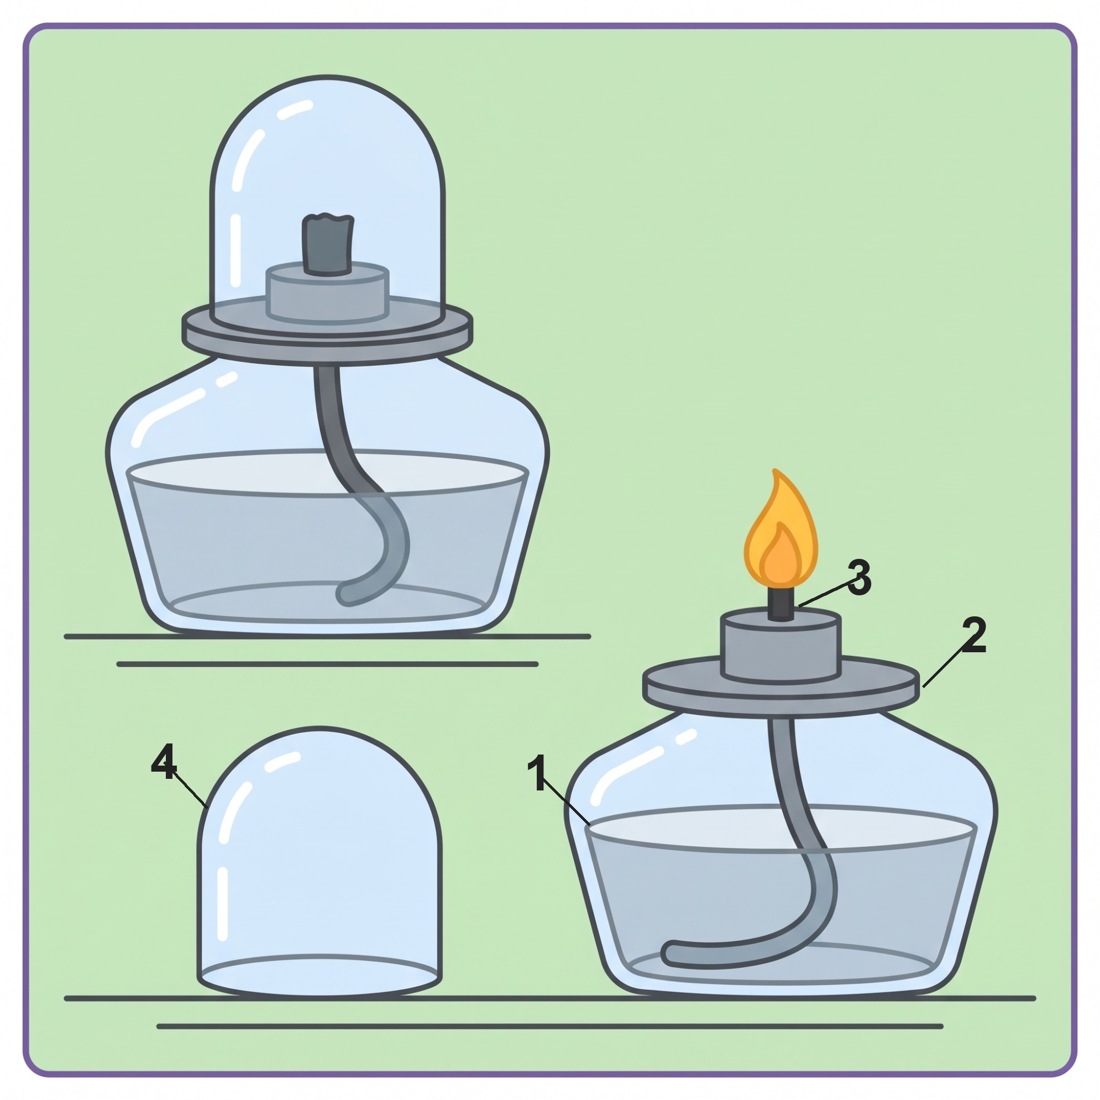
\includegraphics[width=0.86\linewidth]{rasmlar/darslik/d_spirt_lampa.png}\end{center}

\noindent\begin{tabular}{@{}p{0.47\linewidth}@{}p{0.47\linewidth}@{}}
A)~\textsl{qalpoqcha} & B)~\textsl{shtativ} \\
C)~\textsl{metall disk} & D)~\textsl{tutqich} \\
\end{tabular}\par
\qsep
\noindent\qn{31.} Ammoniy xlorid va natriy xlorid eritmalarini (moddalarini) bir-biridan qaysi reagent yordamida farqlash mumkin?
\noindent A)~\textsl{kumush nitrat}\par
\noindent B)~\textsl{natriy gidroksid (qizdirilganda)}\par
\noindent C)~\textsl{xlorid kislota}\par
\noindent D)~\textsl{bariy xlorid}\par
\qsep
\noindent\qn{32.} Laboratoriyada olingan vodorod qanday usulda yig`iladi?
\noindent A)~\textsl{havoni siqib chiqarish (idish og`zi pastga)}\par
\noindent B)~\textsl{havoni siqib chiqarish (idish og`zi yuqoriga)}\par
\noindent C)~\textsl{gazni suyuqlantirib yig`iladi}\par
\noindent D)~\textsl{suvni siqib chiqarish usulida   ---}\par
\qsep
\end{multicols}
\medskip
\noindent\setlength{\fboxsep}{0pt}\fbox{\begin{tabular}{p{0.74\linewidth}|p{0.2\linewidth}}
\parbox[t]{0.72\linewidth}{\vspace{3pt}\textbf{Topshiriqlar (33--35) va javob variant (A--F)larini o`zaro to`g`ri moslashtiring.} 2 mol glyukoza spirtli bijg`ishga uchradi (unum 9/10). Hosil bo`lgan etanolning 1/2 qismi sirka kislotagacha oksidlandi; olingan kislota suvda eritilib, hajmi 18 l bo`lgan eritma tayyorlandi (kislotaning dissotsilanish darajasi 1\%). Shu miqdordagi sirka kislota mo`l NaHCO\textsubscript{3} bilan ham ta'sirlashtirildi.
\vspace{3pt}} & \parbox[t]{0.19\linewidth}{\vspace{3pt}A~\textsl{40,32}\\[3pt]
B~\textsl{165,6}\\[3pt]
C~\textsl{6}\\[3pt]
D~\textsl{3}\\[3pt]
E~\textsl{2,4}\\[3pt]
F~\textsl{20,16}}\\ \hline
\parbox[t]{0.72\linewidth}{\vspace{2pt}\textbf{33. Hosil bo`lgan etanol massasini (g) toping.}\vspace{2pt}} & \\ \hline
\parbox[t]{0.72\linewidth}{\vspace{2pt}\textbf{34. Sirka kislota eritmasining pH ini hisoblang.}\vspace{2pt}} & \\ \hline
\parbox[t]{0.72\linewidth}{\vspace{2pt}\textbf{35. NaHCO\textsubscript{3} bilan ajralgan gazning hajmini (l, n.sh.) aniqlang.}\vspace{2pt}} & 
\end{tabular}}
\par\bigskip
\noindent\qn{36.} Mg + HNO\textsubscript{3} $\to$ Mg(NO\textsubscript{3})\textsubscript{2} + NH\textsubscript{4}NO\textsubscript{3} + H\textsubscript{2}O reaksiya tenglamasini tenglang. Tajriba hajmi 1000 ml bo`lgan kolbada o`tkazildi. Reagentlar (chap qism) koeffitsiyentlari \textbf{yig`indisini toping.}
\javob\qsep
\noindent\qn{37.} 1 l hajmli yopiq idishda 1 mol N\textsubscript{2}O\textsubscript{4} qizdirilganda N\textsubscript{2}O\textsubscript{4} $\rightleftarrows$ 2NO\textsubscript{2} muvozanati qaror topdi. Muvozanat aralashmasining vodorodga nisbatan zichligi 38,33 ga teng. Qizdirish 20 daqiqa davom etdi. Shu haroratdagi muvozanat \textbf{konstantasini (K, mol/l) hisoblang.}
\javob\qsep
\noindent\qn{38.} 12,4 g fosfor yondirib hosil bo`lgan oksid suvda eritildi, so`ng eritmaga 1 mol NaOH qo`shildi (NaOH : H\textsubscript{3}PO\textsubscript{4} = 2,5 : 1). Tajriba 10 daqiqa davom etdi. Hosil bo`lgan tuzlar umumiy \textbf{massasini (g) toping.}
\javob\qsep
\noindent\qn{39.} Etanol va fenoldan iborat 18,6 g aralashma natriy bilan to`liq reaksiyaga kirishganda 3,36 l (n.sh.) vodorod ajraldi. Shu aralashmaga mo`l bromli suv ta'sir ettirilganda hosil bo`ladigan cho`kma \textbf{massasini (g) toping.}
\javob\qsep
\noindent\qn{40.} 37 g etilformiat mo`l NaOH bilan qizdirilganda uning 1/2 qismi gidrolizlandi. Hosil bo`lgan spirt to`liq yondirildi. Qizdirish 20 daqiqa davom etdi. Yondirishda ajralgan CO\textsubscript{2} \textbf{hajmini (l, n.sh.) toping.}
\javob\qsep
\par\bigskip\begin{center}\textbf{\fontsize{13}{15}\selectfont YOZMA ISH}\end{center}
\noindent\qn{41.} \textbf{Topshiriqni bajarish jarayonida barcha reaksiya tenglamalarini yozing. Miqdoriy va arifmetik hisoblashlarni (unga asos bo`lgan usul yoki formulani ko`rsatgan holda) uzviy ketma-ketlikda bajaring.}\par\smallskip
31,6 g KMnO\textsubscript{4} qizdirilganda qisman parchalandi. Ajralgan kislorodning hajmi 27 \textdegree{}C va 83,14 kPa da 1,5 l ga teng bo`ldi (R = 8,314 J/(mol$\cdot$K)). Qizdirish 60 daqiqa davom etdi. Qattiq qoldiq mo`l konsentrlangan xlorid kislota bilan qizdirildi (K\textsubscript{2}MnO\textsubscript{4}, MnO\textsubscript{2} va parchalanmay qolgan KMnO\textsubscript{4} ning barchasi reaksiyaga kirishdi).\par
\noindent 1)\ Parchalanish va qattiq qoldiqning xlorid kislota bilan reaksiyalarini yozing va tenglashtiring (elektron balans).\par
\noindent 2)\ KMnO\textsubscript{4} ning necha foizi parchalanganini aniqlang.\par
\noindent 3)\ Qattiq qoldiq massasini (g) va undagi MnO\textsubscript{2} ning massa ulushini (\%) toping.\par
\noindent 4)\ Ajralgan xlorning umumiy hajmini (l, n.sh.) va sarflangan HCl miqdorini (mol) hisoblang.\par
\noindent 5)\ Reaksiyadan so`ng eritmadagi tuzlarning (KCl va MnCl\textsubscript{2}) umumiy massasini (g) toping.\par
\diqqat{Mazkur topshiriq kengaytirilgan javobni talab etib, uning yechilish usuli va shu usul asosidagi barcha hisoblash amallari javoblar varaqasida aks etishi lozim.}\qsep
\noindent\qn{42.} Organik moddalarning xossalarini bilgan holda reaksiya tenglamalarini tugallang va tenglashtiring. 3- va 5-reaksiyalarda hosil bo`lgan asosiy organik mahsulotlarni sistematik nomenklatura bo`yicha nomlang. Hosil bo`lgan organik moddalarning tuzilish formulalarini yozing.\par
\noindent 1)\ CH\textsubscript{3}--C$\equiv$CH + 2HCl $\to$\par
\noindent 2)\ CH\textsubscript{3}--CH\textsubscript{2}--CHO + Ag\textsubscript{2}O (NH\textsubscript{3}, t) $\to$\par
\noindent 3)\ H\textsubscript{2}N--CH\textsubscript{2}--COOH + H\textsubscript{2}N--CH\textsubscript{2}--COOH $\to$\par
\noindent 4)\ C\textsubscript{6}H\textsubscript{5}--CH\textsubscript{3} + Cl\textsubscript{2} (yorug`lik) $\to$\par
\noindent 5)\ C\textsubscript{6}H\textsubscript{5}--NH\textsubscript{2} + Br\textsubscript{2} (suvli eritma) $\to$\par
\noindent 6)\ H\textsubscript{2}N--CH\textsubscript{2}--COOH + HCl $\to$\par
\noindent 7)\ CH\textsubscript{3}--CH\textsubscript{2}--CH(OH)--CH\textsubscript{3} (H\textsubscript{2}SO\textsubscript{4} kons., t) $\to$\par
\diqqat{Mazkur topshiriq kengaytirilgan javobni talab etib, uning yechilish usuli va shu usul asosidagi barcha hisoblash amallari javoblar varaqasida aks etishi lozim.}\qsep
\noindent\qn{43.} \textbf{Topshiriqni bajarish jarayonida barcha reaksiya tenglamalarini yozing. Miqdoriy va arifmetik hisoblashlarni (unga asos bo`lgan usul yoki formulani ko`rsatgan holda) uzviy ketma-ketlikda bajaring.}\par\smallskip
NH\textsubscript{4}Cl va (NH\textsubscript{4})\textsubscript{2}SO\textsubscript{4} dan iborat 22,65 g aralashmaning bir porsiyasi mo`l NaOH eritmasi bilan qizdirilganda 8,96 l (n.sh.) gaz ajraldi. Xuddi shunday massali ikkinchi porsiya suvda eritilib, mo`l BaCl\textsubscript{2} eritmasi bilan ta'sirlashtirildi. Birinchi porsiyadan ajralgan gaz 0,25 mol H\textsubscript{3}PO\textsubscript{4} saqlagan eritmaga to`liq yuttirildi (NH\textsubscript{4}H\textsubscript{2}PO\textsubscript{4} va (NH\textsubscript{4})\textsubscript{2}HPO\textsubscript{4} aralashmasi hosil bo`ldi). Hosil bo`lgan fosfat tuzlari aralashmasi mo`l NaOH bilan qizdirilganda ajralgan gaz 300 g suvga yuttirildi va olingan eritma 10\% li HCl eritmasi bilan to`liq neytrallandi.\par
\noindent 1)\ Barcha reaksiyalarning tenglamalarini yozing va tenglashtiring. Dastlabki aralashmadagi tuzlarning massalarini (g) aniqlang.\par
\noindent 2)\ Ikkinchi porsiyada hosil bo`lgan cho`kma massasini (g) hisoblang.\par
\noindent 3)\ Fosfat kislotaga yuttirilganda hosil bo`lgan tuzlarning mol miqdorlarini toping. Fosfat tuzlari aralashmasi NaOH bilan qizdirilganda ajralgan gazning hajmini (l, n.sh.) toping.\par
\noindent 4)\ Hosil bo`lgan fosfat tuzlari aralashmasining massasini (g) va undagi azot massa ulushini (\%) aniqlang. Gaz 300 g suvga yuttirilganda eritmadagi moddaning massa ulushini (\%) hisoblang.\par
\noindent 5)\ Birinchi porsiyada ishlatilgan NaOH ning minimal massasini (g) hisoblang. Eritmani neytrallash uchun sarflangan 10\% li HCl eritmasining massasini (g) aniqlang.\par
\diqqat{Mazkur topshiriq kengaytirilgan javobni talab etib, uning yechilish usuli va shu usul asosidagi barcha hisoblash amallari javoblar varaqasida aks etishi lozim.}\qsep
\newpage
\noindent\textbf{\fontsize{13}{15}\selectfont 2-variant}\hfill \textbf{Javoblar kaliti}\par\smallskip\hrule\smallskip
\textit{Faqat o`qituvchi uchun.}\par\medskip
\noindent\textbf{1--32-savollar}\par\smallskip
\noindent\begin{tabular}{|c|c|c|c|c|c|c|c|c|c|c|c|c|c|c|c|}\hline
\textbf{1} & \textbf{2} & \textbf{3} & \textbf{4} & \textbf{5} & \textbf{6} & \textbf{7} & \textbf{8} & \textbf{9} & \textbf{10} & \textbf{11} & \textbf{12} & \textbf{13} & \textbf{14} & \textbf{15} & \textbf{16}\\\hline
\textsl{A} & \textsl{D} & \textsl{C} & \textsl{A} & \textsl{B} & \textsl{C} & \textsl{B} & \textsl{D} & \textsl{D} & \textsl{B} & \textsl{C} & \textsl{D} & \textsl{D} & \textsl{A} & \textsl{D} & \textsl{D}\\\hline
\textbf{17} & \textbf{18} & \textbf{19} & \textbf{20} & \textbf{21} & \textbf{22} & \textbf{23} & \textbf{24} & \textbf{25} & \textbf{26} & \textbf{27} & \textbf{28} & \textbf{29} & \textbf{30} & \textbf{31} & \textbf{32}\\\hline
\textsl{B} & \textsl{C} & \textsl{A} & \textsl{A} & \textsl{B} & \textsl{C} & \textsl{C} & \textsl{C} & \textsl{B} & \textsl{C} & \textsl{A} & \textsl{B} & \textsl{A} & \textsl{A} & \textsl{B} & \textsl{D}\\\hline
\end{tabular}\par\medskip
\noindent\textbf{33--35-savollar}\par\smallskip
\noindent\begin{tabular}{|c|c|c|}\hline \textbf{No} & \textbf{Javob} & \textbf{Qiymat}\\\hline
33 & \textsl{B} & 165,6\\\hline
34 & \textsl{D} & 3\\\hline
35 & \textsl{A} & 40,32\\\hline
\end{tabular}\par\medskip
\noindent\textbf{36--40-savollar}\par\smallskip
\noindent\begin{tabular}{|c|c|}\hline \textbf{No} & \textbf{To`g`ri javob}\\\hline
36 & 14\\\hline
37 & 0,2\\\hline
38 & 61,2\\\hline
39 & 33,1\\\hline
40 & 11,2\\\hline
\end{tabular}\par\medskip
\noindent\textbf{41--43-topshiriqlar: javoblar}\par\smallskip
\noindent\textbf{41-topshiriq.}\par
\noindent 1) 2KMnO\textsubscript{4} $\to$ K\textsubscript{2}MnO\textsubscript{4} + MnO\textsubscript{2} + O\textsubscript{2}$\uparrow$; K\textsubscript{2}MnO\textsubscript{4} + 8HCl $\to$ 2KCl + MnCl\textsubscript{2} + 2Cl\textsubscript{2} + 4H\textsubscript{2}O; MnO\textsubscript{2} + 4HCl $\to$ MnCl\textsubscript{2} + Cl\textsubscript{2} + 2H\textsubscript{2}O; 2KMnO\textsubscript{4} + 16H\par
\noindent 2) 50\%\par
\noindent 3) 30 g; 14,5\%\par
\noindent 4) 8,96 l; 1,4 mol\par
\noindent 5) 40,1 g\par
\noindent\textbf{42-topshiriq.}\par
\noindent 1) CH\textsubscript{3}--C$\equiv$CH + 2HCl $\to$ CH\textsubscript{3}--CCl\textsubscript{2}--CH\textsubscript{3}\par
\noindent 2) CH\textsubscript{3}--CH\textsubscript{2}--CHO + Ag\textsubscript{2}O $\to$ CH\textsubscript{3}--CH\textsubscript{2}--COOH + 2Ag$\downarrow$\par
\noindent 3) 2H\textsubscript{2}N--CH\textsubscript{2}--COOH $\to$ H\textsubscript{2}N--CH\textsubscript{2}--CO--NH--CH\textsubscript{2}--COOH + H\textsubscript{2}O --- nomi: \textbf{glitsilglitsin (dipeptid)}\par
\noindent 4) C\textsubscript{6}H\textsubscript{5}--CH\textsubscript{3} + Cl\textsubscript{2} $\to$ C\textsubscript{6}H\textsubscript{5}--CH\textsubscript{2}Cl + HCl\par
\noindent 5) C\textsubscript{6}H\textsubscript{5}--NH\textsubscript{2} + 3Br\textsubscript{2} $\to$ C\textsubscript{6}H\textsubscript{2}Br\textsubscript{3}--NH\textsubscript{2}$\downarrow$ + 3HBr --- nomi: \textbf{2,4,6-tribromanilin}\par
\noindent 6) H\textsubscript{2}N--CH\textsubscript{2}--COOH + HCl $\to$ [H\textsubscript{3}N--CH\textsubscript{2}--COOH]Cl\par
\noindent 7) CH\textsubscript{3}--CH\textsubscript{2}--CH(OH)--CH\textsubscript{3} $\to$ CH\textsubscript{3}--CH=CH--CH\textsubscript{3} + H\textsubscript{2}O (Zaysev qoidasi)\par
\noindent\textbf{43-topshiriq.}\par
\noindent 1) 16,05 g; 6,6 g\par
\noindent 2) 11,65 g\par
\noindent 3) 0,1 mol; 0,15 mol; 8,96 l\par
\noindent 4) 31,3 g; 17,89\%; 2,22\%\par
\noindent 5) 16 g; 146 g\par
\par\bigskip\noindent\textbf{Mavzular taqsimoti}\par\smallskip
{\small\noindent\begin{longtable}{|c|p{7.2cm}|p{5.4cm}|c|}\hline \textbf{No} & \textbf{Mavzu} & \textbf{Tekshiriladigan ko`nikma} & \textbf{Ball}\\\hline
1 & 8-sinf (davriy qonun, diagramma) & Grafik tahlili & 1\\\hline
2 & Tirkashev I bob; 8-sinf (izoelektron) & Bilim va tushunish & 1\\\hline
3 & 11-sinf (yadro reaksiyalari) & Rasm bo`yicha tahlil & 1\\\hline
4 & 8-sinf (atom tuzilishi, jadval) & Jadval tahlili & 1\\\hline
5 & Tirkashev VI bob & Hisoblash va masala yechish & 1\\\hline
6 & 9-sinf; 11-sinf (tuzlar gidrolizi; Le-Shatelye) & Bilim va tushunish & 1\\\hline
7 & Tashev; 9-sinf (metallarning kuchlanish qatori) & Hisoblash va masala yechish & 1\\\hline
8 & 9-sinf (metallarning kislotalar bilan reaksiyasi) & Hisoblash va masala yechish & 1\\\hline
9 & 8-sinf (ekvivalentlar qonuni) & Hisoblash va masala yechish & 1\\\hline
10 & 8-9-sinf (eritmalar; ketma-ket jarayon) & Hisoblash va masala yechish & 1\\\hline
11 & Tirkashev VI bob (tezlik, jadval) & Jadval tahlili & 1\\\hline
12 & Tirkashev III bob (oleum); Tashev & Hisoblash va masala yechish & 1\\\hline
13 & Tirkashev VI bob (muvozanat, jadval) & Jadval tahlili & 1\\\hline
14 & 9-sinf (ishqoriy metallar); Tashev & Bilim va tushunish & 1\\\hline
15 & 9-sinf; 11-sinf (amfoter birikmalar, kompleks hosil bo`lishi) & Bilim va tushunish & 1\\\hline
16 & 8-9-sinf (eritmalar; bug`latish) & Hisoblash va masala yechish & 1\\\hline
17 & 9-sinf; Tashev (temir) & Hisoblash va masala yechish & 1\\\hline
18 & 9-sinf (suvning qattiqligi va uni yumshatish) & Hisoblash va masala yechish & 1\\\hline
19 & 9-sinf (azot oksidlari; gaz hajmlari) & Hisoblash va masala yechish & 1\\\hline
20 & 10-sinf (nomenklatura \S{}6, \S{}11, \S{}20, \S{}24--26) & Bilim va tushunish & 1\\\hline
21 & 10-sinf (mavzuga oid paragraflar); Abdusamatov & Bilim va tushunish & 1\\\hline
22 & 10-sinf (mavzuga oid paragraflar); Abdusamatov & Bilim va tushunish & 1\\\hline
23 & 10-sinf (uglevodlar; glukozaning bijg`ishi) & Hisoblash va masala yechish & 1\\\hline
24 & 10-sinf (aldegidlarning kumush ko`zgu reaksiyasi) & Hisoblash va masala yechish & 1\\\hline
25 & 10-sinf (alkenlarni gidrogenlash) & Hisoblash va masala yechish & 1\\\hline
26 & 10-sinf (aminlar va anilin xossalari) & Hisoblash va masala yechish & 1\\\hline
27 & 10-sinf (uglevodlar: kraxmal, glukoza) & Hisoblash va masala yechish & 1\\\hline
28 & 10-sinf (arenlar, anilin) & Hisoblash va masala yechish & 1\\\hline
29 & 10-sinf (karbon kislotalar; chumoli kislotaning o`ziga xosligi) & Hisoblash va masala yechish & 1\\\hline
30 & 7-sinf (laboratoriya jihozlari, 3-rasm) & Rasm bo`yicha tahlil & 1\\\hline
31 & 9-sinf; 10-sinf (sifat reaksiyalari; moddalarni farqlash) & Bilim va tushunish & 1\\\hline
32 & 9--10-sinf (gazlarni yig`ish) & Bilim va tushunish & 1\\\hline
33--35 & Aralash masala (moslashtirish) & Ko`p bosqichli hisob & 3\\\hline
36--40 & Qisqa javobli masalalar & Hisoblash & 5\\\hline
41--43 & Yozma ish & Usul va hisob (M, A) & 75\\\hline
\end{longtable}}
\end{document}
